% chapters/chapter1/sec4.tex

\section{Review of Prerequisite Knowledge: Core Principles of Digital Communication and Radar Sensing}
\label{sec:ch1-prerequisites}
 

\subsection{Purpose of This Section}
\label{subsec:ch1-prerequisites-purpose}

% TODO:
% 1. Explain why a review of prerequisite knowledge is needed;
% 2. Clarify the scope and boundary of this section;
% 3. Explain the relationship between this section and the subsequent ISAC chapters.

Text to be added.

\subsection{Core Principles of Digital Communication}
\label{subsec:ch1-digital-comm}


 
\noindent\textbf{Basic Link of a Digital Communication System}


In a digital communication system,
information transmission is not simply the process of sending a signal from the transmitter to the receiver.
Instead,
it is a systematic process centered on the reliable recovery of information bits.
The transmitter first converts the information to be transmitted into an electromagnetic signal
that is suitable for propagation over the wireless channel.
The receiver then needs to recover the original information bits from the received signal
as accurately as possible under unfavorable conditions such as noise,
fading,
multipath propagation,
and interference.
Therefore,
from the communication perspective,
the core objective of system design can be summarized as follows:
to achieve reliable and efficient information transmission under limited bandwidth,
limited power,
and complex wireless environments.

This basic link is also the starting point for understanding ISAC.
ISAC does not construct an independent sensing system outside the communication system.
Instead,
it further exploits the sensing capability of wireless signals on the basis of an existing communication link.
In other words,
the same transmitted signal can carry communication bits,
and it may also carry environmental or target information through propagation,
reflection,
and reception.
Therefore,
before discussing ISAC,
it is necessary to clarify the basic components of a digital communication link
and how these components provide the foundation for subsequent joint waveform design,
channel modeling,
MIMO beamforming,
and resource optimization.

Fig.~\ref{fig:communication_chain} shows a basic block diagram of a typical digital communication system.
The purpose of this diagram is not to cover all details of a communication system.
Rather,
it is intended to help readers build the minimum necessary understanding of the link:
how information bits are converted into wireless signals,
how the signal propagates through the channel,
and how the receiver recovers information from the distorted signal.
\begin{figure}[htbp]
    \centering
    \resizebox{0.92\textwidth}{!}{
    \begin{tikzpicture}[
        block/.style={
            rectangle,
            draw=black,
            thick,
            fill=white,
            minimum width=2.1cm,
            minimum height=0.9cm,
            align=center,
            font=\sffamily\normalsize
        },
        arrow/.style={
            ->,
            >=Stealth,
            thick
        },
        label_text/.style={
            font=\sffamily\small,
            align=center
        }
    ]

    % ------------------------------------------------
    % Transmitter
    % ------------------------------------------------
    \node[block] (source) at (0,0) {Source};
    \node[block] (src_enc) at (2.8,0) {Source\\Coding};
    \node[block] (chn_enc) at (5.6,0) {Channel\\Coding};
    \node[block] (mod) at (8.4,0) {Modulation};

    \node[
        draw,
        dashed,
        thick,
        inner sep=10pt,
        fit=(source) (src_enc) (chn_enc) (mod)
    ] (tx_box) {};

    \node[
        above=0.12cm of tx_box.north,
        font=\sffamily\large\bfseries
    ] {Transmitter};

    % ------------------------------------------------
    % Channel
    % ------------------------------------------------
    \node[block] (channel) at (8.4,-2.3) {Wireless\\Channel};

    \node[
        label_text,
        left=1.3cm of channel
    ] (noise) {Noise/\\Interference};

    \draw[arrow, dashed, gray] (noise) -- (channel);

    % ------------------------------------------------
    % Receiver
    % ------------------------------------------------
    \node[block] (recv) at (8.4,-4.6) {Reception};
    \node[block] (demod) at (5.6,-4.6) {Demodulation};
    \node[block] (dec) at (2.8,-4.6) {Decoding};
    \node[block] (sink) at (0,-4.6) {Destination};

    \node[
        draw,
        dashed,
        thick,
        inner sep=10pt,
        fit=(recv) (demod) (dec) (sink)
    ] (rx_box) {};

    \node[
        below=0.12cm of rx_box.south,
        font=\sffamily\large\bfseries
    ] {Receiver};

    % ------------------------------------------------
    % Connections
    % ------------------------------------------------
    \draw[arrow] (source) -- (src_enc);
    \draw[arrow] (src_enc) -- (chn_enc);
    \draw[arrow] (chn_enc) -- (mod);

    \draw[arrow] (mod) -- 
        node[midway, right, font=\sffamily\small] {RF signal}
        (channel);

    \draw[arrow] (channel) -- 
        node[midway, right, font=\sffamily\small, align=center] {Distorted\\signal}
        (recv);

    \draw[arrow] (recv) -- (demod);
    \draw[arrow] (demod) -- (dec);
    \draw[arrow] (dec) -- (sink);

    \end{tikzpicture}
    }
    \caption{Basic link diagram of a digital communication system}
    \label{fig:communication_chain}
\end{figure}
\begin{itemize}
    \item \textbf{Information source:}
    The information source generates the raw information to be transmitted.
    In a digital communication system,
    this information can usually be abstracted as a raw bit sequence.
    For example,
    text,
speech,
images,
or sensor data need to be represented as discrete digital bits
    before entering the communication system.

    \item \textbf{Source coding:}
    The main role of source coding is to compress redundancy in the information
    and improve the efficiency of information representation.
    After source coding,
    the raw information is converted into a more compact information bit stream,
    so as to reduce the resource overhead required for subsequent transmission.

    \item \textbf{Channel coding:}
    The main role of channel coding is to enhance the reliability of the communication system.
    It introduces controlled redundancy into the information bits,
    so that the receiver can detect and correct a certain level of transmission errors
    in the presence of noise,
fading,
and interference.
    Therefore,
    the bits after channel coding are also often referred to as coded bits.

    \item \textbf{Modulation:}
    The role of modulation is to map discrete coded bits into modulation symbols
    suitable for wireless transmission,
    and further form an RF signal for transmission.
    Common modulation schemes include PSK and QAM.
    In an ISAC system,
    the modulation waveform affects not only the transmission efficiency of communication data,
    but also the ability to estimate range,
velocity,
and angle in sensing tasks.

    \item \textbf{Wireless channel:}
    The wireless channel describes the changes experienced by an RF signal during spatial propagation.
    During propagation,
    the signal is affected by path loss,
multipath fading,
noise,
and interference.
    Therefore,
    the signal obtained at the receiver is a distorted signal after channel distortion
    and noise superposition.
    For ISAC,
    the wireless channel not only affects communication quality,
    but also carries sensing information related to the environment,
targets,
and propagation paths.

    \item \textbf{Reception:}
    The reception module obtains the received signal from the wireless channel
    and performs front-end processing such as down-conversion,
sampling,
and synchronization.
    The received signal contains the useful signal,
noise,
interference,
and channel propagation effects.
    In an ISAC system,
    the received signal may also contain echo information generated by reflections from targets or the environment.

    \item \textbf{Demodulation:}
    The role of demodulation is to estimate the modulation symbols sent by the transmitter
    based on the received signal,
    and further obtain the corresponding soft information or hard-decision bits.
    Since the signal is affected by noise and interference in the wireless channel,
    demodulation results may contain decision errors.
    Therefore,
    subsequent channel decoding is still needed to further improve reliability.

    \item \textbf{Decoding:}
    The decoding module recovers the original information bits according to the channel coding rule
    adopted at the transmitter,
    using the soft information or hard-decision bits output by the demodulator.
    The goal of decoding is to correct transmission errors as much as possible,
    so that the information recovered at the receiver is as close as possible to the transmitted information.

    \item \textbf{Destination:}
    The destination is the final endpoint of information transmission.
    It receives the information recovered after decoding
    and uses it for subsequent data processing,
display,
storage,
or control tasks.
\end{itemize}
From the perspective of ISAC,
the most important components are the modulation waveform,
the wireless channel,
the antenna array,
and the received-signal processing chain.
This is because the sensing function usually does not act directly on the ``bits'' themselves.
Instead,
it exploits the environmental information carried by wireless signals during propagation and reflection.
For example,
the transmitted waveform determines the range and velocity resolution,
the channel response contains the spatial characteristics of targets or the environment,
and received-signal processing determines whether the system can extract sensing parameters
while recovering communication information.
Therefore,
the digital communication link is not only the basis of information transmission,
but also the physical carrier that enables the integration of communication and sensing in ISAC.


\paragraph{Basic Signal Model of a Communication System}

In a communication system,
the transmitted signal experiences fading and multipath spreading after passing through the wireless channel,
and noise or interference is also added.
The time-domain baseband model can be written as
\begin{equation}
    y(t) = h(t) * x(t) + n(t),
    \label{eq:comm_time_domain_model}
\end{equation}
where \(x(t)\) is the transmitted baseband signal,
\(h(t)\) is the impulse response of the wireless channel,
\(n(t)\) is noise or interference,
\(y(t)\) is the received signal,
and \(*\) denotes convolution.
This model indicates that the signal observed at the receiver is the result of the joint effect
of the transmitted signal,
the channel,
and noise.

After the Fourier transform,
the above convolution relationship can be written as a multiplicative form in the frequency domain:
\begin{equation}
    Y(f) = H(f)X(f) + N(f).
    \label{eq:comm_frequency_domain_model}
\end{equation}
The frequency-domain model provides an intuitive description of how different frequency components
are affected differently by the channel,
and it lays the foundation for understanding OFDM multi-carrier transmission
and frequency-domain resource allocation.

In discrete-time,
multi-carrier,
or multi-antenna systems,
the communication link is also often written in a unified form as
\begin{equation}
    \mathbf{Y} = \mathbf{H}\mathbf{X} + \mathbf{N},
    \label{eq:comm_matrix_model}
\end{equation}
where \(\mathbf{X}\) denotes the transmitted-signal representation generated from information bits
after coding and modulation,
\(\mathbf{H}\) denotes the discrete channel response or channel matrix,
\(\mathbf{N}\) denotes noise or interference,
and \(\mathbf{Y}\) denotes the received-signal representation.
This form is very common in MIMO,
OFDM,
and multi-user communication systems,
and it also provides a unified mathematical basis for subsequent joint waveform design,
channel modeling,
and receiver processing in ISAC systems.

\paragraph{Basic Signal Model of an ISAC System}

In a traditional communication system,
the transmitted signal mainly serves as the physical carrier of information bits.
Its core task is to be correctly demodulated and decoded at the receiver
after transmission through the wireless channel.
In an ISAC system,
however,
the same transmitted signal has a richer role:
it not only needs to carry communication information,
but also illuminates targets or the environment during propagation,
and carries information about the external physical world through reflection,
scattering,
and related processes.
Therefore,
the ISAC signal model needs to describe both the communication reception process
and the sensing echo process.

To reflect this dual function,
the received signal in an ISAC system can be divided into communication observation
and sensing observation.
For the communication function,
the received signal can still be written in a form similar to that of traditional communication:
\begin{equation}
    \mathbf{Y}_{\mathrm{C}}
    =
    \mathbf{H}\mathbf{X}
    +
    \mathbf{N}_{\mathrm{C}},
    \label{eq:isac_communication_model}
\end{equation}
where \(\mathbf{X}\) denotes the ISAC transmitted signal,
\(\mathbf{H}\) denotes the communication channel matrix,
\(\mathbf{N}_{\mathrm{C}}\) denotes noise or interference at the communication receiver,
and \(\mathbf{Y}_{\mathrm{C}}\) denotes the communication received signal.
In this case,
the receiver focuses on how to recover the information bits carried by \(\mathbf{X}\)
from \(\mathbf{Y}_{\mathrm{C}}\).

For the sensing function,
the same transmitted signal \(\mathbf{X}\) illuminates the target or the environment
and generates a sensing echo.
The sensing reception model can be written as
\begin{equation}
    \mathbf{Y}_{\mathrm{R}}
    =
    \mathbf{G}\mathbf{X}
    +
    \mathbf{N}_{\mathrm{R}},
    \label{eq:isac_sensing_model}
\end{equation}
where \(\mathbf{Y}_{\mathrm{R}}\) denotes the echo signal obtained by the sensing receiver,
\(\mathbf{G}\) denotes the target response matrix,
also referred to as the sensing channel in this context,
and \(\mathbf{N}_{\mathrm{R}}\) denotes the noise at the sensing receiver.
Unlike the communication channel \(\mathbf{H}\),
\(\mathbf{G}\) describes not only the signal propagation process,
but is also closely related to target or environmental parameters,
such as target range,
velocity,
angle,
reflection coefficient,
and scattering characteristics.
Therefore,
the sensing receiver does not focus on recovering information bits,
but on estimating target or environmental parameters from \(\mathbf{Y}_{\mathrm{R}}\).

From the above models,
it can be seen that the key difference between ISAC and traditional communication systems
is not merely the addition of a sensing receiver.
Rather,
the same transmitted signal \(\mathbf{X}\) is assigned a dual role:
for communication users,
\(\mathbf{X}\) is the carrier of information bits;
for sensing tasks,
\(\mathbf{X}\) is the illumination signal for probing targets and the environment.
Correspondingly,
the communication channel \(\mathbf{H}\) mainly serves information transmission,
whereas the target response matrix \(\mathbf{G}\) serves environmental sensing
and parameter estimation.

Therefore,
the basic signal model of ISAC can be understood as a natural extension
of the traditional communication model.
The traditional communication model emphasizes how to reliably transmit information through the channel,
whereas the ISAC model further emphasizes how to use the same wireless signal
to achieve information transmission and environmental sensing at the same time.
This point also forms the basis for subsequent discussions of joint waveform design,
MIMO beamforming,
the trade-off between communication and sensing performance,
and resource optimization.


\bigskip
\noindent\textbf{Basic Concepts of Wireless Channels and Communication Quality}

The previous part established basic signal models from the perspectives of both communication systems
and ISAC systems.
In an ISAC system,
the communication observation and the sensing observation can be written as
\[
    \mathbf{Y}_{\mathrm{C}}
    =
    \mathbf{H}\mathbf{X}
    +
    \mathbf{N}_{\mathrm{C}},
\]
\[
    \mathbf{Y}_{\mathrm{R}}
    =
    \mathbf{G}\mathbf{X}
    +
    \mathbf{N}_{\mathrm{R}}.
\]
These two models show that the same transmitted signal \(\mathbf{X}\)
plays different roles in communication and sensing tasks.
For the communication receiver,
\(\mathbf{X}\) is the signal carrying information bits,
and the communication channel \(\mathbf{H}\) determines whether the receiver can reliably recover the information.
For the sensing receiver,
\(\mathbf{X}\) is the probing signal that illuminates targets or the environment,
and the target response matrix or sensing channel \(\mathbf{G}\)
contains information related to range,
velocity,
angle,
reflection characteristics,
and other physical properties.
The noise or interference terms \(\mathbf{N}_{\mathrm{C}}\) and \(\mathbf{N}_{\mathrm{R}}\)
further affect the accuracy of communication demodulation and sensing parameter estimation.

It can therefore be seen that the wireless channel is not an ideal,
stable,
or transparent transmission pipe.
Instead,
it is a complex environment jointly affected by propagation distance,
blockage,
multipath reflection,
user mobility,
noise,
and external interference.
For communication systems,
these factors directly determine the received signal quality
and further affect performance metrics such as BER,
throughput,
and spectral efficiency.
For ISAC systems,
they not only affect the reliability of the communication link,
but may also carry sensing information related to targets,
the environment,
and propagation paths.
Therefore,
after understanding the basic signal models,
it is necessary to further review the main influencing factors in wireless channels,
communication quality metrics,
and the role of channel state information,
so as to lay the foundation for understanding OFDM,
MIMO beamforming,
and ISAC joint design.
 
\paragraph{Path Loss}

When a wireless signal propagates in space,
the received power usually decreases as the propagation distance increases.
This average power attenuation caused by the propagation process is called path loss.
Path loss describes the most basic propagation trend in a wireless channel:
under otherwise identical conditions,
the farther the transmitter and receiver are from each other,
the lower the signal power that can usually be obtained at the receiver.

Under ideal free-space propagation conditions,
the received power is commonly described by the Friis transmission formula:
\begin{equation}
    P_r
    =
    P_t G_t G_r
    \left(
        \frac{\lambda}{4\pi d}
    \right)^2 .
    \label{eq:friis-transmission}
\end{equation}
Here,
\(P_t\) denotes the transmit power,
\(P_r\) denotes the received power,
\(G_t\) and \(G_r\) denote the transmit antenna gain and receive antenna gain,
respectively,
\(\lambda\) denotes the signal wavelength,
and \(d\) denotes the propagation distance between the transmitter and the receiver.
From Eq.~\eqref{eq:friis-transmission},
it can be seen that the received power is related not only to the transmit power and antenna gains,
but also closely to the propagation distance and the signal wavelength.
When the propagation distance \(d\) increases,
the received power \(P_r\) decreases.
When the signal frequency becomes higher and the wavelength \(\lambda\) becomes shorter,
the received power also decreases under the same propagation distance.

From Eq.~\eqref{eq:friis-transmission},
it can be further seen that the attenuation caused by free-space propagation is mainly determined by the factor
\[
    \left(
        \frac{\lambda}{4\pi d}
    \right)^2
\]
If the power loss caused by the propagation process itself is represented separately,
the free-space path loss can be written as
\begin{equation}
    \mathrm{FSPL}(d)
    =
    \left(
        \frac{4\pi d}{\lambda}
    \right)^2 .
    \label{eq:free-space-path-loss-linear}
\end{equation}
In engineering analysis,
path loss is usually expressed in dB form as
\begin{equation}
    \mathrm{FSPL}_{\mathrm{dB}}(d)
    =
    20\log_{10}
    \left(
        \frac{4\pi d}{\lambda}
    \right).
    \label{eq:free-space-path-loss-db}
\end{equation}
Accordingly,
the received power in a link budget can also be written as
\begin{equation}
    P_r(\mathrm{dBm})
    =
    P_t(\mathrm{dBm})
    +
    G_t(\mathrm{dB})
    +
    G_r(\mathrm{dB})
    -
    \mathrm{FSPL}_{\mathrm{dB}}(d).
    \label{eq:link-budget-fspl}
\end{equation}
Eq.~\eqref{eq:link-budget-fspl} more intuitively illustrates the role of path loss
in a communication link:
transmit power and antenna gains increase the received power,
whereas path loss reduces the received power.

It should be noted that the free-space path loss model is an idealized model.
It assumes a clear line-of-sight propagation path between the transmitter and the receiver,
and does not consider complex environmental factors such as building blockage,
ground reflection,
scatterers,
and diffraction.
In practical urban,
indoor,
industrial,
and vehicular-network scenarios,
the wireless propagation environment is more complex.
The received signal strength is also affected by blockage,
multipath propagation,
material reflection properties,
antenna height,
and other factors.
Therefore,
path loss mainly describes the average trend of received signal strength with distance,
whereas rapid local fluctuations need to be further explained together with multipath propagation
and fading phenomena.

\paragraph{Multipath Propagation}

In a practical wireless environment,
the transmitted signal usually does not reach the receiver along only one path.
In addition to the direct path,
the signal may also be reflected,
scattered,
or diffracted by buildings,
the ground,
walls,
vehicles,
human bodies,
or other scatterers,
and then arrive at the receiver from different directions and with different propagation distances.
The phenomenon in which the same transmitted signal forms multiple signal copies through multiple propagation paths
and these copies arrive jointly at the receiver is called multipath propagation.
It should be noted that multipath propagation does not mean that there are multiple independent transmitted signals.
Rather,
it means that the same transmitted signal is ``decomposed'' by the wireless environment during propagation
into multiple components with different delays,
amplitudes,
phases,
and angles of arrival.

In a relatively simple time-invariant multipath channel,
the channel impulse response can be written as
\begin{equation}
    h(\tau)
    =
    \sum_{\ell=1}^{L}
    \alpha_{\ell}
    \delta
    \left(
        \tau-\tau_{\ell}
    \right),
    \label{eq:time-invariant-multipath-channel}
\end{equation}
where
\(L\) denotes the number of resolvable propagation paths,
\(\alpha_{\ell}\) denotes the complex gain of the \(\ell\)-th path,
which describes the amplitude attenuation and phase variation on that path,
\(\tau_{\ell}\) denotes the propagation delay of the \(\ell\)-th path,
and \(\delta(\cdot)\) denotes the impulse function.
Eq.~\eqref{eq:time-invariant-multipath-channel} shows that the signal observed at the receiver
can be understood as the superposition of multiple delayed signal copies.

In mobile communication,
vehicular networks,
low-altitude UAV systems,
and dynamic industrial scenarios,
the transmitter,
the receiver,
or scatterers in the environment may change with time.
In this case,
the multipath channel also becomes time-varying.
More generally,
a time-varying multipath channel can be expressed as
\begin{equation}
    h(t,\tau)
    =
    \sum_{\ell=1}^{L}
    \alpha_{\ell}(t)
    \delta
    \left(
        \tau-\tau_{\ell}(t)
    \right),
    \label{eq:time-varying-multipath-channel}
\end{equation}
where
\(\alpha_{\ell}(t)\) and \(\tau_{\ell}(t)\)
denote the time-varying complex gain and propagation delay of the \(\ell\)-th path,
respectively.
If mobility is further considered,
each path may also correspond to different Doppler shifts and angle information.
Therefore,
a multipath channel not only has a delay structure,
but may also exhibit variations in the time,
frequency,
and spatial dimensions.

For communication systems,
multipath propagation changes the amplitude,
phase,
and delay structure of the received signal.
Without proper processing,
it may cause signal distortion,
ISI,
or fluctuations in received power.
However,
in multi-antenna systems such as MIMO,
rich scattering and multipath propagation may also increase the degrees of freedom of the spatial channel,
thereby providing conditions for diversity gain and spatial multiplexing.
Therefore,
multipath is not always purely detrimental.
Instead,
it needs to be compensated,
suppressed,
or exploited according to the system structure and design objective.

For ISAC systems,
multipath propagation has a more direct physical meaning.
Different propagation paths often correspond to different targets,
reflectors,
or scattering structures in the real environment.
Thus,
multipath components may carry sensing information such as range,
velocity,
angle,
and reflection characteristics.
For example,
in urban road scenarios,
signals transmitted by a base station or roadside unit may be reflected by vehicles,
buildings,
road surfaces,
and pedestrians.
Some reflected paths may help target localization and environmental sensing,
whereas others may form clutter or false echoes.
It can therefore be seen that multipath in ISAC is not only a channel effect that affects communication quality,
but also an important information source for understanding and sensing the physical environment.

Multipath propagation itself mainly describes the path structure through which the signal arrives at the receiver.
When these path components overlap and vary in time,
frequency,
or space,
the received signal further exhibits different forms of fading.
The next part explains the concept of fading and its basic classifications.


\paragraph{Fading}

Fading in wireless channels refers to the phenomenon in which the amplitude,
phase,
or power of the received signal changes with spatial position,
time,
or frequency.
It is not caused by a single factor.
Instead,
it is the result of the joint effects of propagation distance,
blockage,
multipath propagation,
mobility,
carrier frequency,
and the surrounding environment.
Path loss and shadowing mainly affect the average received signal power.
Coherent superposition of multipath components causes rapid local fluctuations.
The motion of the transmitter,
receiver,
or scatterers makes the channel vary with time.
Therefore,
we understand its physical origins and manifestations from the spatial,
time,
and frequency perspectives.


\noindent\textbullet\quad\textbf{From the spatial scale: large-scale fading and small-scale fading}

\textbf{Large-scale fading} refers to the variation of the average received signal power over a relatively large spatial range.
It is mainly caused by path loss and shadowing.
For example,
when a user gradually moves away from the base station,
the received power usually decreases as the propagation distance increases.
When the signal propagation path is blocked by obstacles such as buildings,
trees,
or vehicles,
the received power may also drop significantly.
Large-scale fading reflects the average variation trend of a wireless link over a large spatial scale,
and is usually closely related to coverage,
link budget,
and shadowing.

\textbf{Small-scale fading} refers to the rapid fluctuation of the received signal over a short time interval
or a short spatial distance.
It is mainly caused by the coherent superposition of multipath components.
Because different propagation paths have different propagation distances,
phases,
and delays,
these components may reinforce or cancel each other when they are superimposed at the receiver.
Therefore,
even if the receiver moves only a very short distance,
the received signal may be significantly strengthened or weakened.
Compared with large-scale fading,
small-scale fading focuses more on the rapid local fluctuations caused by multipath superposition.

As shown in Fig.~\ref{fig:spatial-fading},
large-scale fading is mainly reflected as the average decreasing trend of received power with increasing distance,
whereas small-scale fading appears as local rapid fluctuations superimposed on this average trend.

\begin{figure}[htbp]
    \centering
    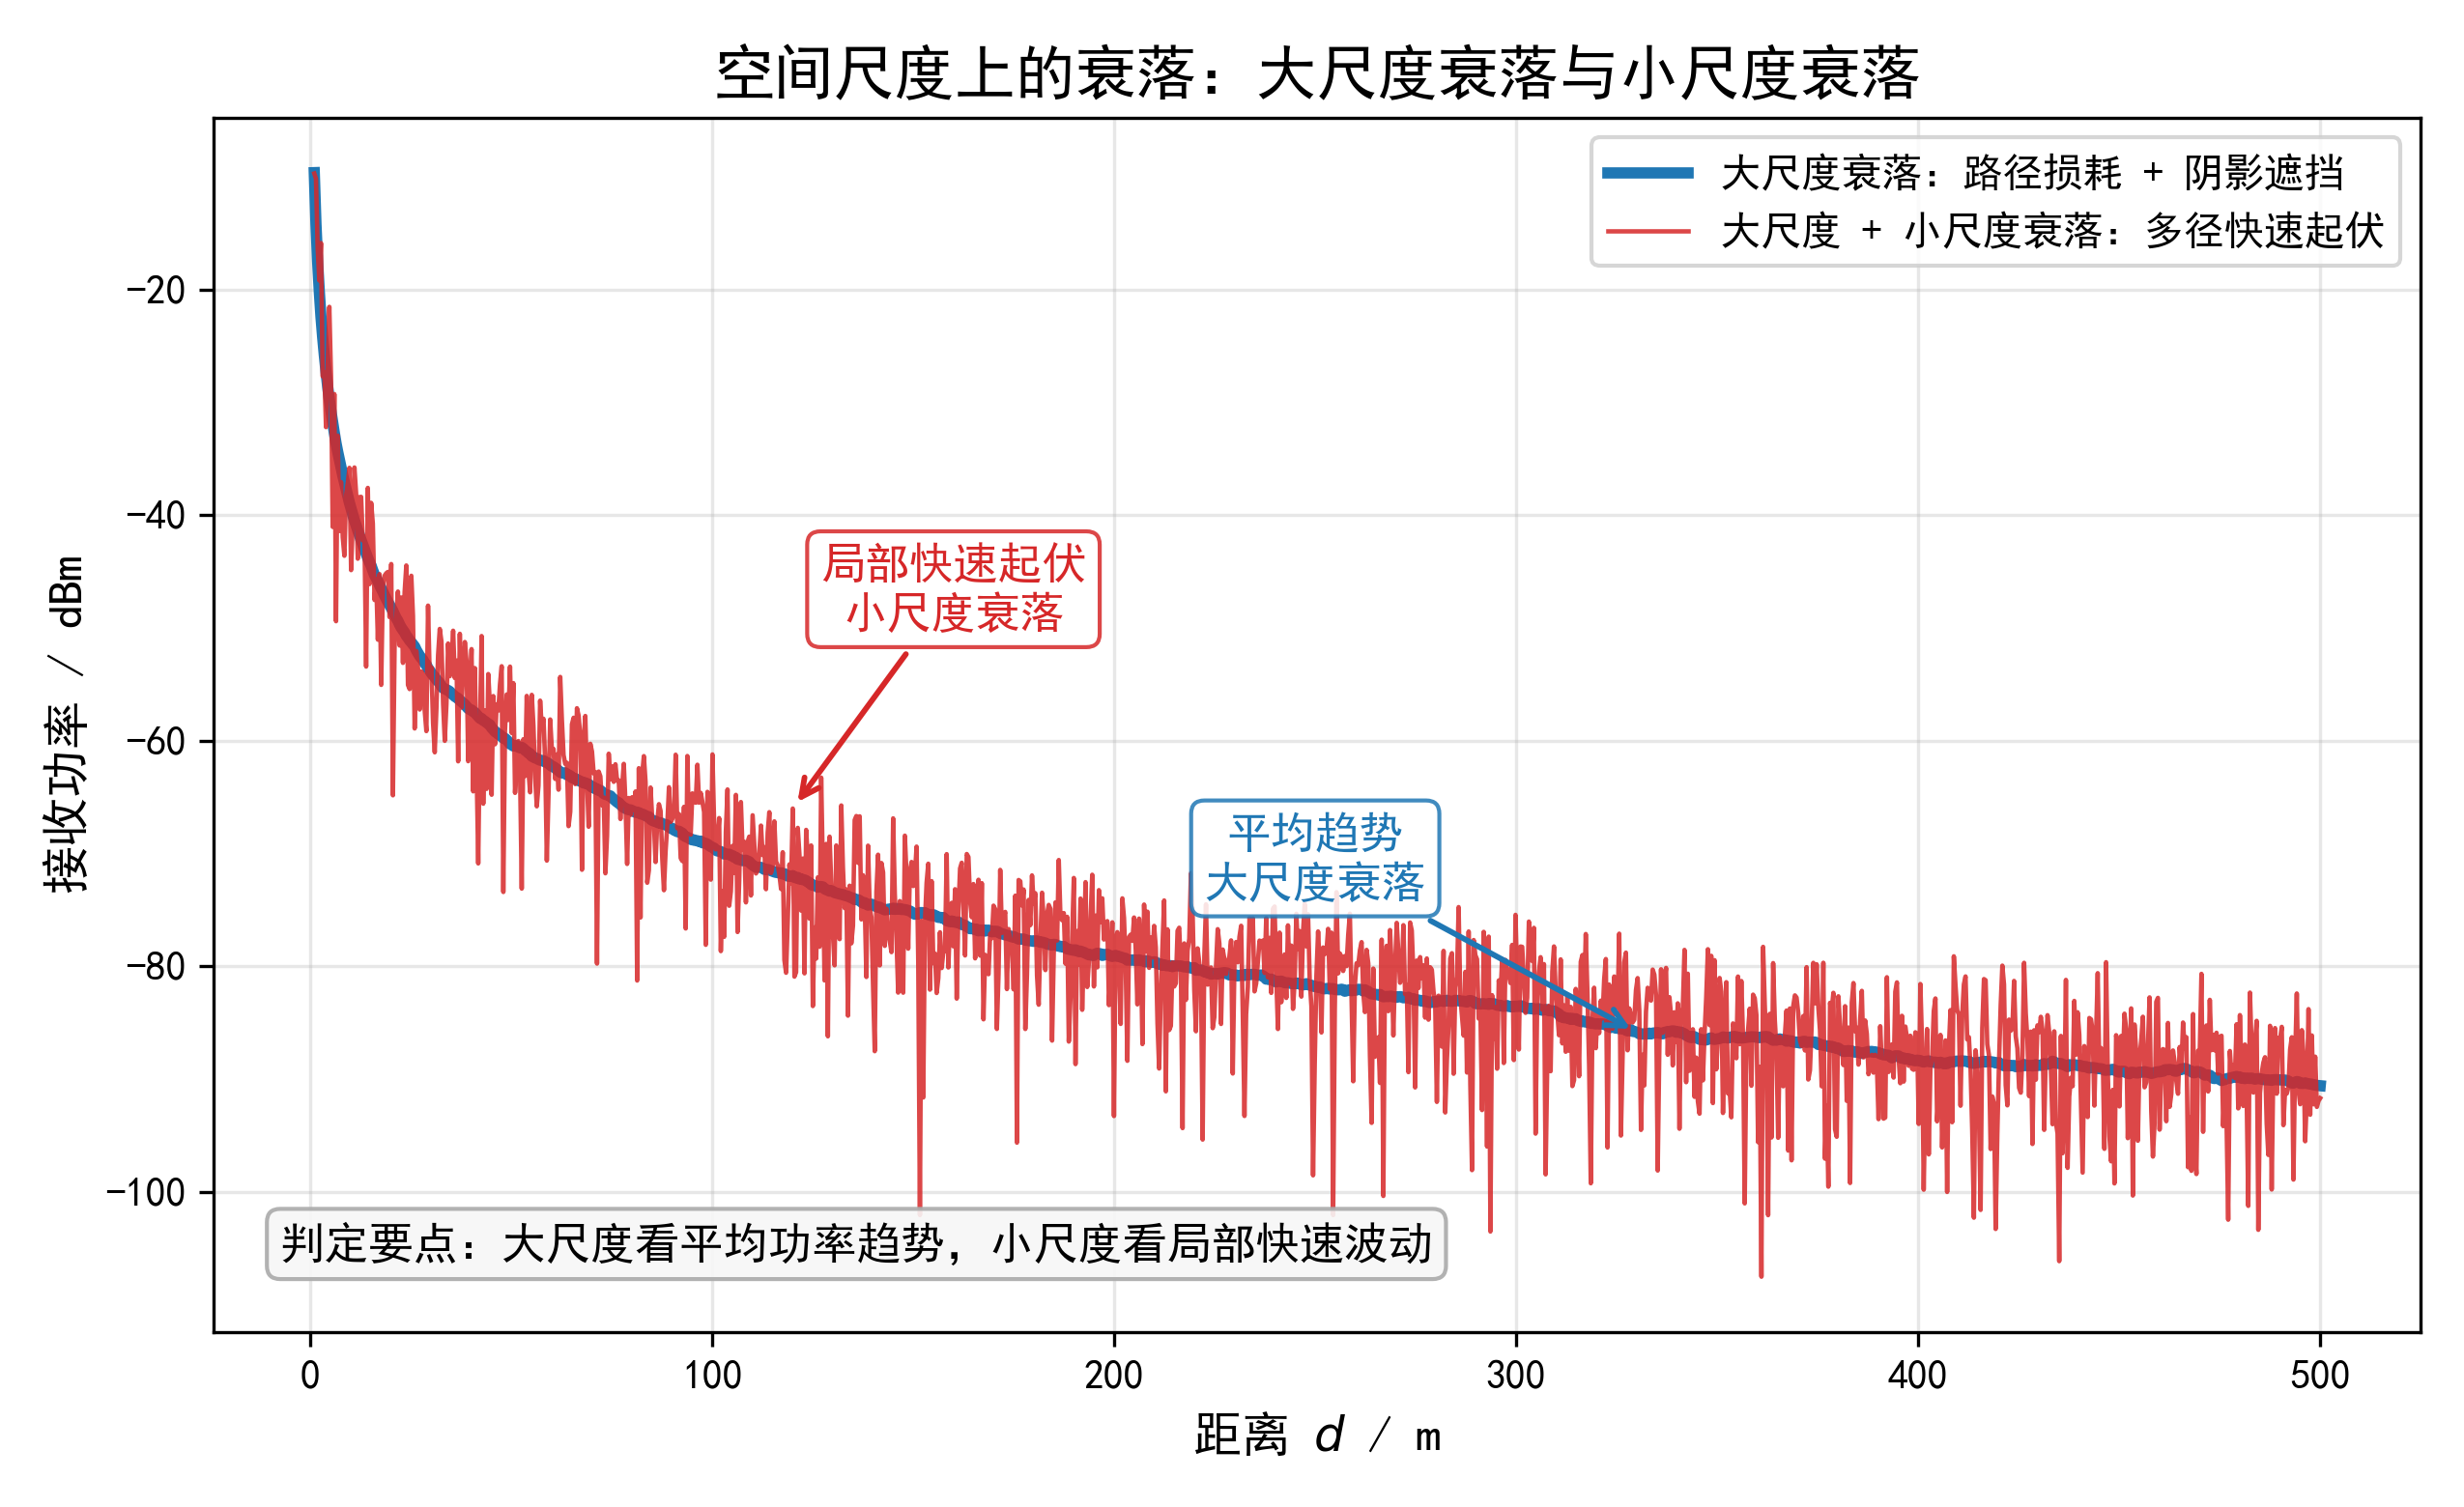
\includegraphics[width=0.75\textwidth]{figures/chapter1/fig_fading.png}
    \caption{Comparison between large-scale fading and small-scale fading}
    \label{fig:spatial-fading}
\end{figure}
\noindent\textbullet\quad\textbf{From the time dimension: Doppler shift, coherence time, and fast/slow fading}

From the time dimension,
fading is closely related to the time-varying characteristics of the channel.
When there is relative motion among the transmitter,
receiver,
or scatterers in the environment,
the amplitude and phase of each propagation path may vary with time,
so that the channel exhibits non-stationary or time-varying characteristics.
In particular,
the phase variation caused by relative motion appears as a Doppler shift.
The maximum Doppler shift is usually written as
\begin{equation}
    f_D
    =
    \frac{v}{\lambda}
    =
    \frac{v f_c}{c},
    \label{eq:maximum-doppler-shift}
\end{equation}
where
\(v\) denotes the relative velocity,
\(\lambda\) denotes the carrier wavelength,
\(f_c\) denotes the carrier frequency,
and \(c\) denotes the speed of light.
From Eq.~\eqref{eq:maximum-doppler-shift},
it can be seen that,
for the same carrier frequency,
a higher relative velocity leads to a larger Doppler shift.
For the same moving speed,
a higher carrier frequency and a shorter wavelength make the Doppler effect more significant.
Therefore,
the time variation of the channel becomes more prominent in high-mobility scenarios
and high-frequency communication scenarios such as millimeter-wave and terahertz systems.

To describe the temporal stability of the channel,
the concept of \textbf{coherence time} \(T_c\) is usually introduced.
Coherence time can be understood as the time scale over which the channel remains approximately unchanged.
In general,
coherence time is approximately inversely proportional to the maximum Doppler shift,
namely
\begin{equation}
    T_c
    \propto
    \frac{1}{f_D}.
    \label{eq:coherence-time}
\end{equation}
A larger Doppler shift leads to a shorter coherence time,
which indicates that the channel varies faster.
A smaller Doppler shift leads to a longer coherence time,
which indicates that the channel remains more stable over a longer period.

Based on this concept,
the difference between slow fading and fast fading can be understood.
Let the symbol duration of the signal be \(T_s\).

\textbf{Slow fading} refers to the case where the channel varies slowly relative to the signal.
If \(T_s \ll T_c\),
the channel remains almost unchanged within one symbol duration,
and the received signal can be approximately regarded as passing through a relatively fixed channel.
In this case,
the channel variation mainly occurs over a longer time scale,
and this is usually called slow fading.

\textbf{Fast fading} refers to the case where the channel varies rapidly relative to the signal.
If \(T_s\) is close to \(T_c\),
or even larger than \(T_c\),
the channel may change significantly within one symbol duration,
so that the received signal experiences time-varying channel effects even inside a symbol.
In this case,
synchronization,
channel estimation,
and equalization at the receiver become more difficult,
and this is usually called fast fading.

Therefore,
fast fading and slow fading are not absolute concepts determined only by whether the moving speed is high.
Rather,
they are determined by the relative relationship between the time scale of channel variation
and the time scale of the signal.

\noindent\textbullet\quad\textbf{From the frequency dimension: delay spread, coherence bandwidth, and frequency selectivity}

From the frequency dimension,
fading is closely related to multipath delay spread.
In multipath propagation,
different paths have different propagation distances,
so their arrival times at the receiver are not exactly the same.
The phenomenon in which multiple path components spread along the delay axis is called delay spread.
The root-mean-square delay spread \(\tau_{\mathrm{rms}}\) is commonly used
to describe the dispersion of multipath energy along the delay axis.
A larger delay spread means that the arrival-time differences among different multipath components are more significant,
and the fluctuations of the channel frequency response with frequency are usually stronger.

To describe the correlation range of the channel in frequency,
the concept of \textbf{coherence bandwidth} \(B_c\) is usually introduced.
Coherence bandwidth can be understood as the frequency range over which the channel frequency response remains approximately consistent.
In general,
coherence bandwidth is approximately inversely proportional to the root-mean-square delay spread,
namely
\begin{equation}
    B_c
    \propto
    \frac{1}{\tau_{\mathrm{rms}}}.
    \label{eq:coherence-bandwidth}
\end{equation}
A larger delay spread leads to a smaller coherence bandwidth,
which means that the channel may vary significantly even over a narrower frequency range.
A smaller delay spread leads to a larger coherence bandwidth,
which means that the channel response may remain similar over a wider frequency band.

\textbf{Flat fading} refers to the fading condition in which the signal bandwidth \(B\)
is much smaller than the coherence bandwidth \(B_c\),
namely \(B \ll B_c\).
In this case,
all frequency components within the signal bandwidth experience approximately the same channel response,
and the entire signal band can be approximately regarded as being affected by a single complex channel coefficient.
Therefore,
although flat fading changes the overall amplitude and phase of the signal,
it usually does not cause significantly different distortions among different frequency components.

\textbf{Frequency-selective fading} refers to the fading condition in which the signal bandwidth \(B\)
is close to the coherence bandwidth \(B_c\),
or \(B > B_c\).
In this case,
different frequency components may experience different amplitude attenuations and phase variations,
so the received signal exhibits non-uniform distortion in the frequency domain.
Frequency-selective fading is an important problem in wideband wireless communication,
and it is also one of the main motivations for OFDM multi-carrier transmission.
OFDM divides a wideband signal into multiple narrowband subcarriers,
so that the channel on each subcarrier approximately behaves as a flat-fading channel,
thereby reducing the complexity of equalization and receiver processing.

It should be emphasized that large-scale fading,
small-scale fading,
slow fading,
fast fading,
flat fading,
and frequency-selective fading are not mutually exclusive classifications.
They describe the variation characteristics of wireless channels from different observation perspectives:
the spatial scale focuses on the trend of the received signal with position,
the time dimension focuses on how fast the channel varies with time,
and the frequency dimension focuses on how the channel affects different frequency components differently.
A practical wireless channel may be affected simultaneously by path loss,
shadowing,
multipath superposition,
mobility,
and frequency selectivity.

For traditional communication systems,
fading is mainly regarded as an adverse factor that affects reliable transmission and link quality.
For ISAC systems,
however,
the physical quantities behind fading,
such as delay,
Doppler,
angle,
and path gain,
may also carry sensing information about target motion,
spatial structure,
and environmental state.
Therefore,
in ISAC,
understanding fading is not only for compensating channel effects,
but also for further exploiting environmental information in the wireless propagation process.

The above fading concepts describe different characteristics of wireless channels
from the perspectives of spatial scale,
time variation,
and frequency response.
For ease of comparison and memorization,
Table~\ref{tab:fading-types-comparison} summarizes the main sources,
criteria,
and intuitive meanings of common fading types.
In practical wireless environments,
these fading phenomena often coexist
and jointly affect the communication link quality and the sensing performance of ISAC systems.
\begin{table}[htbp]
    \centering
    \caption{Comparison of different fading types}
    \label{tab:fading-types-comparison}
    \renewcommand{\arraystretch}{1.35}
    \begin{tabularx}{\textwidth}{p{0.13\textwidth} p{0.16\textwidth} X X X}
        \hline
        \textbf{Observation Perspective}
        &
        \textbf{Fading Type}
        &
        \textbf{Main Source}
        &
        \textbf{Criterion}
        &
        \textbf{Intuitive Meaning}
        \\
        \hline

        Spatial scale
        &
        Large-scale fading
        &
        Path loss, shadowing, terrain and building blockage
        &
        Average received signal power varies slowly with position or distance
        &
        The overall signal becomes weaker or is blocked
        \\

        Spatial scale
        &
        Small-scale fading
        &
        Coherent superposition of multipath components
        &
        The received signal fluctuates rapidly over a short distance or a short time
        &
        Moving only a short distance may significantly strengthen or weaken the signal
        \\

        Time dimension
        &
        Slow fading
        &
        Low mobility and small Doppler shift
        &
        \(T_s \ll T_c\)
        &
        The channel is approximately unchanged within one symbol duration
        \\

        Time dimension
        &
        Fast fading
        &
        High mobility, large Doppler shift, or rapidly varying scattering environment
        &
        \(T_s \gtrsim T_c\)
        &
        The channel has already changed significantly within one symbol duration
        \\

        Frequency dimension
        &
        Flat fading
        &
        Small multipath delay spread
        &
        \(B \ll B_c\)
        &
        Frequency components within the whole signal bandwidth experience approximately the same channel
        \\

        Frequency dimension
        &
        Frequency-selective fading
        &
        Large multipath delay spread
        &
        \(B \gtrsim B_c\)
        &
        Different frequency components experience different amplitude attenuations and phase variations
        \\
        \hline
    \end{tabularx}
\end{table}


\paragraph{Classification of Communication Quality Metrics}

The path loss,
multipath propagation,
fading,
noise,
and interference discussed above all change the signal quality observed at the receiver.
To evaluate the impact of these factors on information transmission,
a communication system needs to introduce a series of quality metrics.
Different metrics focus on different levels.
Some metrics describe the quality of the received signal itself,
some measure whether information recovery is reliable,
and others reflect how much useful information the system can transmit under limited spectrum and time resources.
Therefore,
communication quality metrics can be roughly divided into three categories:
\textbf{link quality metrics},
\textbf{reliability metrics},
and \textbf{efficiency metrics}.

\textbf{Link quality metrics} are mainly used to describe the strength of the useful signal
relative to noise or interference at the receiver.
Typical metrics include the signal-to-noise ratio (SNR)
and the signal-to-interference-plus-noise ratio (SINR).
The SNR is defined as the ratio between useful signal power and noise power,
namely
\begin{equation}
    \mathrm{SNR}
    =
    \frac{P_s}{P_n},
    \label{eq:snr-definition}
\end{equation}
where
\(P_s\) denotes the useful signal power at the receiver,
and \(P_n\) denotes the noise power.
If the noise power spectral density is \(N_0\)
and the system bandwidth is \(B\),
the noise power can often be written as
\begin{equation}
    P_n
    =
    N_0 B.
    \label{eq:noise-power-bandwidth}
\end{equation}
Therefore,
when the received signal power is fixed,
an increase in bandwidth introduces more noise power,
which may reduce the SNR.
In general,
higher transmit power,
smaller path loss,
and larger antenna gain or beamforming gain lead to stronger received signal power
and a higher SNR;
larger noise power leads to a lower SNR.

In practical systems,
the undesired components at the receiver often include not only noise,
but also interference from other users,
neighboring cells,
co-channel systems,
or spectrum-sharing devices.
Therefore,
SINR is more suitable than SNR for describing the actual communication link quality.
It is defined as
\begin{equation}
    \mathrm{SINR}
    =
    \frac{P_s}{P_i + P_n},
    \label{eq:sinr-definition}
\end{equation}
where
\(P_i\) denotes the interference power.
When the interference power is small,
SINR approximately reduces to SNR.
When the system is interference-limited,
communication performance may improve only slightly even if the transmit power is increased.
In this case,
interference coordination,
resource scheduling,
power control,
and beamforming become more important.
For ISAC systems,
the meaning of SINR is even more important,
because communication and sensing functions may share time,
frequency,
space,
and power resources.
Communication signals,
sensing echoes,
clutter,
and signals from other users may form more complex interactions.

\textbf{Reliability metrics} are used to measure whether the receiver can correctly recover the information sent by the transmitter.
The most common reliability metric is the bit error rate (BER),
which is defined as the ratio between the number of erroneous bits and the total number of transmitted bits:
\begin{equation}
    \mathrm{BER}
    =
    \frac{N_{\mathrm{error}}}{N_{\mathrm{total}}},
    \label{eq:ber-definition}
\end{equation}
where
\(N_{\mathrm{error}}\) denotes the number of bits incorrectly decided at the receiver,
and \(N_{\mathrm{total}}\) denotes the total number of transmitted bits.
A lower BER indicates higher communication link reliability.
Usually,
a higher SNR or SINR makes it easier for the receiver to distinguish different modulation symbols,
thereby reducing the BER.
When fading is severe,
interference becomes stronger,
or noise power increases,
the BER often increases.

The bit error rate is also closely related to the modulation scheme and channel coding.
Under the same SNR condition,
higher-order modulation can carry more bits in each symbol,
but the distance between constellation points becomes smaller.
Therefore,
it is usually more susceptible to noise and interference.
Lower-order modulation has lower spectral efficiency,
but stronger robustness.
Channel coding can help the receiver detect and correct errors by introducing redundancy,
thereby reducing the BER,
but it also introduces a certain rate overhead.
In practical mobile communication systems,
the block error rate (BLER) is also commonly used
to describe whether a transport block is correctly decoded.
Compared with BER,
BLER is closer to the evaluation needs of link adaptation,
retransmission mechanisms,
and actual throughput.

\textbf{Efficiency metrics} are used to measure the capability of a communication system
to transmit information under limited resources.
The most basic rate metric is the data rate,
which denotes the number of information bits transmitted per unit time.
In an ideal Gaussian channel,
the channel capacity can be used as a theoretical upper-bound reference,
which is given by
\begin{equation}
    C
    =
    B \log_2
    \left(
        1+\mathrm{SNR}
    \right),
    \label{eq:capacity-snr}
\end{equation}
where
\(C\) denotes the channel capacity,
and \(B\) denotes the system bandwidth.
If interference is considered,
SNR is often replaced by SINR,
and the capacity can be written as
\begin{equation}
    C
    =
    B \log_2
    \left(
        1+\mathrm{SINR}
    \right).
    \label{eq:capacity-sinr}
\end{equation}
Eq.~\eqref{eq:capacity-snr} and Eq.~\eqref{eq:capacity-sinr} show that capacity is related to both bandwidth
and link quality.
Increasing bandwidth provides more frequency resources,
while increasing SNR or SINR improves the amount of information that can be carried per unit bandwidth.
However,
capacity increases logarithmically with SNR or SINR.
Therefore,
in the high-SNR region,
the rate gain brought by further increasing power gradually diminishes.

Throughput is closer to the amount of information successfully transmitted in a practical system.
It can be understood as the amount of useful data correctly received per unit time,
and is commonly written as
\begin{equation}
    R_{\mathrm{throughput}}
    =
    \frac{N_{\mathrm{success}}}{T},
    \label{eq:throughput-definition}
\end{equation}
where
\(N_{\mathrm{success}}\) denotes the number of information bits successfully received within time \(T\).
If \(R\) denotes the nominal transmission rate
and BLER denotes the block error rate,
the actual throughput can be approximately written as
\begin{equation}
    R_{\mathrm{throughput}}
    \approx
    R
    \left(
        1-\mathrm{BLER}
    \right).
    \label{eq:throughput-bler}
\end{equation}
This expression indicates that a higher nominal rate does not necessarily mean a higher actual throughput.
If the channel condition is poor,
leading to a higher error rate or retransmission probability,
the amount of successfully transmitted data may even decrease.

Spectral efficiency is used to measure how much information can be transmitted per unit bandwidth,
and is usually defined as
\begin{equation}
    \eta
    =
    \frac{R}{B},
    \label{eq:spectral-efficiency-definition}
\end{equation}
with the unit bit/s/Hz.
If channel capacity is used as an ideal reference,
spectral efficiency can be written as
\begin{equation}
    \eta
    =
    \log_2
    \left(
        1+\mathrm{SNR}
    \right),
    \label{eq:spectral-efficiency-snr}
\end{equation}
or,
when interference is considered,
as
\begin{equation}
    \eta
    =
    \log_2
    \left(
        1+\mathrm{SINR}
    \right).
    \label{eq:spectral-efficiency-sinr}
\end{equation}
A higher spectral efficiency means that the system has a stronger ability
to transmit information within limited spectrum resources.
Against the background of increasingly scarce spectrum resources,
spectral efficiency is one of the important metrics for evaluating wireless communication systems.
For ISAC,
spectral efficiency has a more specific meaning:
ISAC aims to support information transmission and environmental sensing at the same time
by sharing spectrum,
hardware,
and waveform resources between communication and sensing,
without occupying a large amount of additional spectrum.
Therefore,
spectral efficiency not only reflects the resource utilization capability of the communication link itself,
but is also closely related to communication-sensing resource reuse
and the overall system efficiency.

In practical systems,
there is a clear logical relationship among these communication quality metrics.
Path loss,
multipath,
fading,
noise,
and interference first affect the SNR or SINR at the receiver.
The SNR or SINR then determines the reliability of demodulation and decoding,
which is reflected in metrics such as BER or BLER.
Reliability further affects the actual throughput.
Under a given bandwidth,
the effective transmission rate further determines the spectral efficiency.
Therefore,
communication quality metrics can be understood as layered measures
from ``received signal quality''
to ``information recovery reliability''
and then to ``resource utilization efficiency.''
For ISAC systems,
these metrics remain the basis for evaluating communication performance.
At the same time,
they also provide an important basis for subsequent discussions of the trade-off between communication and sensing performance,
resource allocation,
and joint optimization.

\paragraph{Channel State Information: Definition, Acquisition, and Role}

If a communication system needs to perform receiver processing and transmission optimization
according to the wireless channel state,
it must first obtain descriptive information about the current channel.
Such information is usually called \textbf{channel state information} (CSI).
CSI reflects the effects of amplitude attenuation,
phase rotation,
delay spread,
frequency selectivity,
and spatial direction that the signal experiences during propagation.
In other words,
CSI can be viewed as a mathematical description of the current state of the wireless channel
from the perspective of the communication system.

The specific form of CSI depends on the system structure.
In a single-antenna narrowband system,
CSI can be simplified as a complex channel coefficient
\begin{equation}
    h
    =
    |h|e^{j\phi},
    \label{eq:csi-siso-coefficient}
\end{equation}
where
\(|h|\) describes the change in signal amplitude,
and \(\phi\) describes the change in signal phase.
In an OFDM system,
CSI is usually represented as the frequency-domain channel response on different subcarriers:
\begin{equation}
    H[k],
    \label{eq:csi-ofdm-subcarrier}
\end{equation}
where
\(k\) denotes the subcarrier index,
and \(H[k]\) describes the channel amplitude and phase variation on the \(k\)-th subcarrier.
In a MIMO system,
CSI is often represented as a channel matrix
\begin{equation}
    \mathbf{H},
    \label{eq:csi-mimo-matrix}
\end{equation}
whose matrix elements describe the spatial channel relationships
between different transmit antennas and receive antennas.
It can therefore be seen that CSI does not have a fixed single form,
but its core role is always to describe the effect of the wireless channel on the transmitted signal.

CSI is usually estimated through pilot signals or reference signals.
The transmitter sends pilot symbols known to the receiver at predefined time,
frequency,
or spatial resource positions.
The receiver then estimates the channel based on the known transmitted values of the pilots
and the corresponding received values.
Under different systems and assumptions,
different channel estimation algorithms can be used,
such as least-squares (LS) estimation,
linear minimum mean square error (LMMSE) estimation,
and methods based on interpolation,
filtering,
or compressed sensing.
In an OFDM system,
CSI often needs to be obtained on multiple pilot subcarriers.
The channel responses at other resource positions are then estimated through frequency-domain or time-domain interpolation.
In a MIMO system,
it is also necessary to estimate the channel matrix between different transmit antennas and receive antennas.

The acquisition method of CSI is also related to the duplexing mode.
In an FDD system,
uplink and downlink usually use different frequency bands,
and the two channels are not exactly the same.
Therefore,
after the receiver estimates the downlink CSI,
it usually needs to feed back channel quality or precoding-related information to the transmitter through a feedback link.
In a TDD system,
uplink and downlink use different time slots in the same frequency band.
Ideally,
the wireless propagation channel has reciprocity.
Thus,
the base station can estimate the channel from uplink pilots
and use it for downlink transmission design.
However,
in practical systems,
channel reciprocity is also affected by mismatches in the RF front ends,
so certain calibration is usually required.

CSI plays a fundamental role in communication system design.
First,
the receiver can use CSI for channel equalization
to compensate for amplitude attenuation,
phase rotation,
and frequency-selective distortion caused by the channel,
thereby improving the reliability of demodulation and decoding.
Second,
the transmitter or system scheduler can perform adaptive modulation and coding according to channel quality.
When the channel condition is good,
higher-order modulation and a higher coding rate can be used to improve the data rate.
When the channel condition is poor,
lower-order modulation and stronger channel coding can be used to guarantee reliability.
In addition,
CSI can also be used for power control,
user scheduling,
resource allocation,
and retransmission strategy design.

In MIMO systems,
the role of CSI is even more prominent.
The transmitter or receiver can design beamforming and precoding weights according to the channel matrix,
so that the transmit energy is concentrated as much as possible toward the target user
while suppressing interference to other users.
For multi-user MIMO systems,
CSI can also help the system determine which users are suitable for spatial multiplexing
on the same time-frequency resource,
thereby improving system capacity and spectral efficiency.
It can be said that CSI is an important foundation for communication systems
to move from fixed transmission toward adaptive transmission.

From the perspective of ISAC,
the meaning of CSI is further extended.
In traditional communication systems,
CSI is mainly used to compensate for channel effects
and improve communication reliability and transmission efficiency.
In ISAC systems,
however,
CSI itself may also contain target and environmental information.
For example,
delay information in the channel may correspond to propagation path length or target range,
Doppler shift may reflect the relative motion of a target or scatterer,
angle information may correspond to target direction or spatial structure,
and path gain and reflection characteristics may reflect target scattering strength
or material properties of the environment.
Therefore,
CSI is not only the basis for adaptive communication link design,
but may also become an important entry point for ISAC systems
to sense the environment and understand the target state.

It can therefore be seen that CSI connects the physical characteristics of the wireless channel
with communication system design.
For communication,
CSI is used to adapt to and compensate for the channel.
For ISAC,
CSI can further help the system extract environmental,
target,
and motion information from channel variations.
This is also a fundamental concept that will be repeatedly used in subsequent discussions of OFDM channel estimation,
MIMO beamforming,
and joint communication-sensing processing.
